\documentclass[english,man]{apa6}

\usepackage{amssymb,amsmath}
\usepackage{ifxetex,ifluatex}
\usepackage{fixltx2e} % provides \textsubscript
\ifnum 0\ifxetex 1\fi\ifluatex 1\fi=0 % if pdftex
  \usepackage[T1]{fontenc}
  \usepackage[utf8]{inputenc}
\else % if luatex or xelatex
  \ifxetex
    \usepackage{mathspec}
    \usepackage{xltxtra,xunicode}
  \else
    \usepackage{fontspec}
  \fi
  \defaultfontfeatures{Mapping=tex-text,Scale=MatchLowercase}
  \newcommand{\euro}{€}
\fi
% use upquote if available, for straight quotes in verbatim environments
\IfFileExists{upquote.sty}{\usepackage{upquote}}{}
% use microtype if available
\IfFileExists{microtype.sty}{\usepackage{microtype}}{}
\usepackage[backend=biber,style=apa,sortcites=true,sorting=nyt,doi,url]{biblatex}
\DeclareLanguageMapping{american}{american-apa}
% 
% Table formatting
\usepackage{longtable, booktabs}
\usepackage{lscape}
% \usepackage[counterclockwise]{rotating}   % Landscape page setup for large tables
\usepackage{multirow}		% Table styling
\usepackage{tabularx}		% Control Column width
\usepackage[flushleft]{threeparttable}	% Allows for three part tables with a specified notes section
\usepackage{threeparttablex}            % Lets threeparttable work with longtable

% Create new environments so endfloat can handle them
% \newenvironment{ltable}
%   {\begin{landscape}\begin{center}\begin{threeparttable}}
%   {\end{threeparttable}\end{center}\end{landscape}}

\newenvironment{lltable}
  {\begin{landscape}\begin{center}\begin{ThreePartTable}}
  {\end{ThreePartTable}\end{center}\end{landscape}}

  \usepackage{ifthen} % Only add declarations when endfloat package is loaded
  \ifthenelse{\equal{\string man}{\string man}}{%
   \DeclareDelayedFloatFlavor{ThreePartTable}{table} % Make endfloat play with longtable
   % \DeclareDelayedFloatFlavor{ltable}{table} % Make endfloat play with lscape
   \DeclareDelayedFloatFlavor{lltable}{table} % Make endfloat play with lscape & longtable
  }{}%



% The following enables adjusting longtable caption width to table width
% Solution found at http://golatex.de/longtable-mit-caption-so-breit-wie-die-tabelle-t15767.html
\makeatletter
\newcommand\LastLTentrywidth{1em}
\newlength\longtablewidth
\setlength{\longtablewidth}{1in}
\newcommand\getlongtablewidth{%
 \begingroup
  \ifcsname LT@\roman{LT@tables}\endcsname
  \global\longtablewidth=0pt
  \renewcommand\LT@entry[2]{\global\advance\longtablewidth by ##2\relax\gdef\LastLTentrywidth{##2}}%
  \@nameuse{LT@\roman{LT@tables}}%
  \fi
\endgroup}


  \usepackage{graphicx}
  \makeatletter
  \def\maxwidth{\ifdim\Gin@nat@width>\linewidth\linewidth\else\Gin@nat@width\fi}
  \def\maxheight{\ifdim\Gin@nat@height>\textheight\textheight\else\Gin@nat@height\fi}
  \makeatother
  % Scale images if necessary, so that they will not overflow the page
  % margins by default, and it is still possible to overwrite the defaults
  % using explicit options in \includegraphics[width, height, ...]{}
  \setkeys{Gin}{width=\maxwidth,height=\maxheight,keepaspectratio}
\ifxetex
  \usepackage[setpagesize=false, % page size defined by xetex
              unicode=false, % unicode breaks when used with xetex
              xetex]{hyperref}
\else
  \usepackage[unicode=true]{hyperref}
\fi
\hypersetup{breaklinks=true,
            pdfauthor={},
            pdftitle={A Meta-Analysis of Expressive Writing on Positive Psychology Variables and Traumatic Stress},
            colorlinks=true,
            citecolor=blue,
            urlcolor=blue,
            linkcolor=black,
            pdfborder={0 0 0}}
\urlstyle{same}  % don't use monospace font for urls

\setlength{\parindent}{0pt}
%\setlength{\parskip}{0pt plus 0pt minus 0pt}

\setlength{\emergencystretch}{3em}  % prevent overfull lines

\ifxetex
  \usepackage{polyglossia}
  \setmainlanguage{}
\else
  \usepackage[english]{babel}
\fi

% Manuscript styling
\captionsetup{font=singlespacing,justification=justified}
\usepackage{csquotes}
\usepackage{upgreek}

 % Line numbering
  \usepackage{lineno}
  \linenumbers


\usepackage{tikz} % Variable definition to generate author note

% fix for \tightlist problem in pandoc 1.14
\providecommand{\tightlist}{%
  \setlength{\itemsep}{0pt}\setlength{\parskip}{0pt}}

% Essential manuscript parts
  \title{A Meta-Analysis of Expressive Writing on Positive Psychology Variables
and Traumatic Stress}

  \shorttitle{Expressive Writing}


  \author{Jeffrey M. Pavlacic\textsuperscript{1}, Erin M. Buchanan\textsuperscript{2}, Nicholas P. Maxwell\textsuperscript{2}, Tabetha G. Hopke\textsuperscript{2}, \& Stefan E. Schulenberg\textsuperscript{1}}

  \def\affdep{{"", "", "", "", ""}}%
  \def\affcity{{"", "", "", "", ""}}%

  \affiliation{
    \vspace{0.5cm}
          \textsuperscript{1} University of Mississippi\\
          \textsuperscript{2} Missouri State University  }

  \authornote{
    \newcounter{author}
    Jeffrey M. Pavlacic is a doctoral candidate at the University of
    Mississippi and a member of the University of Mississippi
    Clinical-Disaster Research Center (UM-CDRC). Erin M. Buchanan is an
    Associate Professor of Psychology at Missouri State University. Nicholas
    P. Maxwell and Tabetha G. Hopke are master's degree candidates at
    Missouri State University. Stefan E. Schulenberg is a Professor of
    Psychology at the University of Mississippi and director of the UM-CDRC.

                      Correspondence concerning this article should be addressed to Jeffrey M. Pavlacic, 205 Peabody Hall, University, MS 38655. E-mail: \href{mailto:jpavlaci@go.olemiss.edu}{\nolinkurl{jpavlaci@go.olemiss.edu}}
                                                        }


  \abstract{Emotional expression has been shown to be beneficial for promoting both
positive psychological and physical health outcomes. Unfortunately,
inhibiting emotions can lead to impairments in physical and
psychological health. James Pennebaker showed that expressive writing is
an effective form of emotional expression, and he and others have used
expressive writing as an experimental manipulation to gauge its
effectiveness in treating a wide variety of health-related and
psychological outcomes. While many studies have been conducted that
examine the effectiveness of expressive writing across such outcomes, a
considerable amount of these studies tend to neglect necessary
considerations such as power and meaningfulness of respective effect
sizes. Four previous meta-analyses have been conducted that examine
expressive writing's effect on psychological outcomes. However, these
studies focus on the experimental versus control group effect size.
Thus, our meta-analysis sought to examine the effectiveness of an
expressive writing intervention on only the experimental conditions in
studies measuring posttraumatic growth, posttraumatic stress, and
quality of life using random effects models. Results indicated a small
overall effect size for posttraumatic stress and negligible to small
effect sizes for posttraumatic growth and quality of life. Implications
for future research design and interpretation of published research are
discussed.}
  \keywords{meta-analysis, positive psychology, expressive writing \\

    
  }





\usepackage{amsthm}
\newtheorem{theorem}{Theorem}
\newtheorem{lemma}{Lemma}
\theoremstyle{definition}
\newtheorem{definition}{Definition}
\newtheorem{corollary}{Corollary}
\newtheorem{proposition}{Proposition}
\theoremstyle{definition}
\newtheorem{example}{Example}
\theoremstyle{definition}
\newtheorem{exercise}{Exercise}
\theoremstyle{remark}
\newtheorem*{remark}{Remark}
\newtheorem*{solution}{Solution}
\begin{document}

\maketitle

\setcounter{secnumdepth}{0}



Emotional expression, especially focusing on negative emotions or
trauma, has been shown to increase both mental and physical health
\autocites{Rachman1980}{Scheff1979}{Esterling1990}{Fawzy1993}{Lieberman2006}.
In contrast, inhibiting repressive thoughts or emotions can be
detrimental to both physical and psychological health
\autocites{Gross1997}{Goldstein1988}{Larson1990a}. Additionally,
repressing or avoiding certain emotions may prevent an individual from
living in accordance with his or her values \autocite{Wilson2009}.
Value-congruent behavior allows individuals to foster a sense of meaning
\autocites{Frankl1959}{Schulenberg2008}. Further, individuals
experiencing traumatic events are more likely to repress thoughts and
feelings about a given traumatic experience \autocite{Bodor2002}.
Generally, preventing the disclosure of harmful thoughts and feelings
can be harmful to individuals, while disclosing these events can reduce
stress and lead to various positive health outcomes, such as with
diabetes \autocite{Bodor2002}, breast cancer related illnesses
\autocite{Stanton2002}, and other physical health conditions.

As a caveat, however, the disclosure or acceptance of harmful thoughts
or emotions can sometimes lead to negative outcomes. Thus, caution
should be used when interpreting results from interventions based on
emotional expression \autocite{Wilson2009}. For example,
\textcite{Brouneus2010} found that truth telling, a form of emotional
expression, caused harm to individuals. However, in general, these
repressive maneuvers have the capability to lead to social concerns,
overall psychological dysfunction, and inhibit people from living in
accordance with their values
\autocites{Frankl1959}{Pennebaker1989}{Pennebaker1986}{Schulenberg2008}{Wilson2009}.
Psychological dysfunction can obviously lead to detrimental effects on
health, including unhealthy everyday life habits, which could lead to
biological problems, especially immune system and neurotransmitter
deficiencies \autocite{Pennebaker1986}. By preventing an individual from
living in accordance with his or her values, emotional inhibition may
prohibit individuals from gaining access to values that are
intrinsically reinforcing. Additionally, living in accordance with
personal values allows the individual to foster a sense of meaning
despite debilitating life circumstances
\autocites{Frankl1959}{Schulenberg2008}. Therefore, it is important to
identify and foster ways in which individuals can effectively express
emotions, thereby improving both physical and psychological health.

\textcite{Pennebaker1986} first showed that emotional expression can be
both experimentally manipulated and have positive benefits to
participants. In their seminal study, they randomly assigned
participants to several writing groups including writing about an
experienced trauma or a neutral event. The group that disclosed both
about their trauma and the emotions surrounding that trauma later showed
a reduction in health visits. Pennebaker has replicated the use of
expressive writing (i.e., a paradigm in which one writes about emotions)
across a number of studies ranging from improving health
\autocites{Pennebaker1988}{Pennebaker1990} to improvements in school
\autocite{Pennebaker1996} and work \autocite{Francis1992}. Others have
expanded this work to show positive effects on mood
\autocite{Schoutrop2002} and asthma \autocite{Smyth1999}; however,
several controlled studies have shown to not replicate
\autocite{Harris2005} or null effects
\autocites{Gidron1996a}{Walker1999a}.

The idea that a brief, controlled writing intervention can have numerous
positive health and psychological benefits can certainly be
controversial, especially when recent studies show contradicting
results. For example, \textcite{Henry2010} found that expressive writing
only benefited a rural population for those individuals surviving breast
cancer, while \textcite{Lancaster2015} found no significant evidence
that expressive writing can be considered an effective approach.
Additionally, \textcite{Brouneus2010} found that truth telling caused
harm to individuals in a forensic setting. Regardless, the concept
remains interesting due to the nature and inexpensive implementation of
expressive writing. Many individuals who have experienced traumatic
events do not wish to disclose their feelings regarding the events with
others. Additionally, those who do not meet diagnostic criteria are
sometimes neglected despite probable suffering \autocite{Wilson2009}.
However, by utilizing expressive writing as a personal method of
treatment, individuals are able to effectively express their emotions
while avoiding talking to another individual or clinician about the
traumatic event \autocite{Smyth1998}. \textcite{Pennebaker1993} found
that experimental conditions assigned to participate in an expressive
writing task generally report more positive changes than those in
control conditions. Some controversy has been observed over whether or
not writing about a formerly disclosed event is more effective than
writing about an undisclosed event. \textcite{Greenberg1992} conducted
an experiment where they separated participants into three groups:
writing about a formerly disclosed trauma, writing about an undisclosed
trauma, and a control group. They found no difference between groups in
effectiveness. However, they did find that those who disclosed more
severe traumas reportedly experienced fewer physical symptoms at follow
up, which suggests that the type of trauma revealed can play a
significant impact on symptom reduction and physical health. From a
meta-analytic perspective, \textcite{Mogk2006} found a non-meaningful
effect size when examining the effect of expressive writing on somatic
health symptoms, psychological health, and miscellaneous outcomes, such
as grades and self-efficacy. These results were in contrast to the
meta-analysis conducted by \textcite{Smyth1998}, which found a medium
overall effect size (\emph{d} = 0.47).

In order to understand why expressive writing is considered to be an
effective, intervention-based approach, one must examine the cognitive
and social processes by which it allows an individual to process
information. \textcite{Pennebaker1990} discovered that individuals who
had benefited from expressive writing attributed their success to ways
in which the intervention allowed them to understand what had happened
to them. Furthermore, in an additional study, \textcite{Pennebaker1993}
conducted a textual analysis on expressive writing content and found
that those who were more successful during the intervention used words
that can be categorized as causation words. Pennebaker attributed these
results as individuals effectively processing the event in their own
minds. Aside from cognitive-processing and inhibition theories, there
are a number of other theories that researchers have used to explain
emotional disclosure. The first theory that warrants explanation is the
social integration model \autocite{Pennebaker2001}. This model discusses
how emotional disclosure can have a positive impact on how people
interact in their environment. This increased environmental interaction
has been shown to have positive benefits on health
\autocite{Frattaroli2006}. Finally, expressive writing parallels
exposure therapy for a variety of phobias and posttraumatic stress
disorder, which suggests that repeatedly exposing oneself to the
seemingly anxious thought or trauma can reduce the anxiety, fear, or
stress associated with that event \autocite{Meshberg-Cohen2014}. Given
that exposure therapy has been shown to be effective for reducing
symptoms of posttraumatic stress \autocite[PTS;][]{Sloan2005}, one would
expect individuals in these studies to experience a reduction in PTS
symptoms after taking part in an expressive writing intervention.
Additionally, \textcite{Wilson2009} discussed how the nonjudgmental
acceptance of emotions leads to positive health benefits by promoting
value-congruent behavior, one of the main facets of Acceptance and
Commitment Therapy. Engaging in value-congruent in the presence of
inevitable human suffering is also the foundation of Logotherapy.
Further, these value-based approaches can be integrated with
orientations dedicated to symptom reduction
\autocites{Frankl1959}{Schulenberg2008}. Enhancing life circumstances
through valued action is important, as it has built the foundation for
modern psychotherapy. Sometimes, however, emotional inhibition prevents
an individual from engaging in such action.

\subsection{Meta-Analytic Techniques}\label{meta-analytic-techniques}

Recent advancements in statistical analyses have allowed researchers the
opportunity to objectively examine the effectiveness of different
psychological interventions on outcome variables
\autocites{Glass1976}{Borenstein2007}{Hedges1982}. Although many studies
produced positive outcomes associated with expressive writing, some of
these studies tend to neglect important questions, the most important of
which is whether or not the effect sizes are meaningful
\autocite{Smyth1998}. Meta-analyses are a technique that allow
researchers to pool studies to examine an overall, weighted, population
effect \autocite{Borenstein2007}. Several meta-analyses of expressive
writing and emotional expression have been explored:
\textcite{Smyth1998}, \textcite{Frisina2004a},
\textcite{Frattaroli2006}, and \textcite{Mogk2006}. These meta-analyses
have laid a foundation for exploring the effects of writing on
psychological outcomes. For our purposes, we used Cohen's
\autocite*{Cohen1988} standards for nomenclature for small (0.20),
medium (0.50), and large (0.80) \emph{d} values, although it is
important to note that Cohen himself suggested that these values should
be based on the area of study. Generally, however, these effect size
criteria are used within the social sciences.

The meta-analysis conducted by \textcite{Smyth1998} found an overall
medium effect size, \emph{d} = 0.47, for the experimental group compared
to the control group. This particular analysis examined the
effectiveness of expressive writing on psychological well-being, general
health, and physical functioning. \textcite{Frisina2004a} expanded these
analyses and found that expressive writing had a small to no effect on
health outcomes, weighted \emph{d} = 0.07 to \emph{d} = 0.21. The
meta-analyses conducted by \textcite{Mogk2006} corroborated findings
from \textcite{Frisina2004a}. Specifically, \textcite{Mogk2006} examined
the effectiveness of expressive writing on somatic health symptoms,
psychological outcomes, grades, and self-efficacy. The meta-analyses
conducted by \textcite{Smyth1998} and \textcite{Frisina2004a} were
relatively small in nature, using only 12-14 studies. The meta-analysis
conducted by \textcite{Mogk2006} included 30 studies. Newer methods of
meta-analysis, including \emph{p}-curve
\autocites{Simonsohn2014}{Simonsohn2015}, \emph{p}-uniform
\autocite{VanAert2016}, PET-PEESE \autocite{Stanley2014}, selection
models \autocite{Vevea1995}, and trim and fill methods
\autocite{Carter2014} allow for better estimation of meta-analytic
effect sizes. These analyses would be best performed by examining each
potential effect separately, rather than averaging effects of each
publication into one study effect size.

Additionally, \textcite{Frattaroli2006} conducted a meta-analysis to
examine the effects of emotional disclosure on a variety of variables
such as psychological health, physiological functioning, reported
health, health behaviors, subjective impact of intervention, and general
functioning/life outcomes. This meta-analysis is different from the meta
conducted by \textcite{Smyth1998} in that it utilizes random effects
modeling in order to calculate effect sizes. The current meta-analysis
includes both random and fixed effects models for comparison. Fixed
effects models assume that all studies assess the same \enquote{true}
population effect size, which may be an untenable assumption across
different assessments and populations \autocite{Borenstein2007}. Random
effects models estimate the mean of a proposed distribution of
population effect sizes, which may vary by subject type or research
design. Overall, \textcite{Frattaroli2006} found a weighted \emph{r}
effect size of .08 for all outcomes combined, which would be considered
small. This meta-analysis included a very large range of studies,
\emph{N} = 146, but individual studies were again collapsed into one
publication effect size, although these effects were also examined
separately by health outcome.

An additional methodological concern of the previous meta-analyses is
the focus on experimental versus control group effect sizes, rather than
emphasizing change for an intervention group. This focus is likely
because of the analyses provided in these publications, especially when
using randomized controlled trial research designs. While this design is
the gold standard for medicine, the effects of comparing control groups
versus experimental groups may mask the usefulness of the change for the
intervention group. For example, a comparison group may increase their
quality of life scores by two points in a controlled study, while the
experimental group increases their quality of life scores by four
points; thus, creating a significant difference in change between the
two groups. This information is valuable, but it does not tell us the
magnitude of the change for the intervention group, wherein four points
might only be a small effect when examined within the group who received
the intervention. This study will focus on changes across time for
groups who received the expressive writing task to determine what size
of effects one might expect given a specific measurement schedule (i.e.,
one to three months, three months to six months, etc.). Additionally, we
will examine the change in effects across measurement time to determine
whether or not effects decrease over time.

Expressive writing tasks fit well within the framework of different
psychological interventions and can be adapted for treatment, which is
why the literature includes a multitude of different studies looking at
a wide variety of outcomes. However, it is important to focus on
individual variables in order to determine the effectiveness of
expressive writing for specific diagnoses and psychopathology. As
previously mentioned, some studies have found long-term benefits of
expressive writing on psychological well-being \autocite{Park2002}.
However, other studies, such as the research completed by
\textcite{Lancaster2015}, found no evidence supporting the utilization
of expressive writing as an effective therapeutic approach. Thus, it is
necessary to evaluate the effectiveness of expressive writing on
specific outcome variables, and we chose to focus specifically on
posttraumatic stress (PTS), posttraumatic growth (PTG), and quality of
life (QOL), in line with the current positive psychology trends. By
focusing on specific outcome variables, rather than specific patient or
study characteristics \autocite[which are covered extensively
in][]{Frattaroli2006}, we can examine how effective writing can be for
changing stress and positive psychology phenomena as described below.
With this knowledge, we can decide whether or not to incorporate this
type of intervention into protocols for certain diagnoses.

\subsection{Posttraumatic Stress}\label{posttraumatic-stress}

Posttraumatic Stress Disorder (PTSD) is a disorder involving reoccurring
thoughts or experiences after a traumatic event or experience
\autocite{AmericanPsychiatricAssociation2013}. The diagnosis is based on
20 symptoms structured into four different subsets. These subsets are as
follows: re-experiencing, avoidance, negative alterations in cognition
and mood, and arousal \autocite{Crespo2016}. PTSD is a concerning
disorder that affects a wide variety of groups, a few of which are
sexual assault survivors \autocite{Klump2008}, Iraq and Afghanistan war
veterans \autocite{Gentes2014}, and those exposed to natural disasters
\autocite{Wang2000}. Research conducted on the effectiveness of
expressive writing on PTSD symptoms has been less successful and shows
outcomes that are not as effective as other studies. While PTSD symptoms
decreased after a written emotional disclosure intervention, this
decrease was not significantly different than a control group change
\autocite{Sloan2011a}. Additionally, the emotional disclosure group
showed greater emotional and heart rate responding, leading the
researchers to conclude that writing may not be effective for treating
PTSD.

\textcite{Blasio2015a} suggested that those meeting the criteria for
moderate PTSD benefit more from expressive writing interventions in
comparison to those with greater PTSD symptoms. They recruited women who
had just given birth and assessed them a few days after experiencing
childbirth along with a three-month follow-up. Results showed that women
who had participated in the expressive writing task had lower depression
and posttraumatic stress symptoms than the group assigned to a neutral
writing condition. Additionally, regression models showed that
expressive writing was significantly linked to a reduction of PTSD
symptoms at all baseline levels. Contradicting the work conducted by
\textcite{Sloan2011a}, these results suggest that expressive writing may
be an effective tool for women managing postpartum distress. However, it
is important to note that only 20 of the 113 women recruited for this
study qualified for a diagnosis of PTSD. This limitation suggests that
those with moderate distress could perhaps benefit more from an
expressive writing intervention than those diagnosed with or meeting the
qualifications for PTSD. It may also explain the differences in results
between the two studies, as \textcite{Sloan2011a} found that those with
a clinical diagnosis of PTSD did not respond to an emotional disclosure
writing task. However, \textcite{Blasio2015a} found that those who
reported mild symptomology better responded to the intervention than
those meeting the criteria for a diagnosis of PTSD. As previously
mentioned, expressive writing mirrors exposure therapy in that it
encourages individuals to express avoided emotions related to the
aversive event. Thus, given this observation, one would expect PTS
scores to decrease in those taking part in an expressive writing
intervention.

\subsection{Posttraumatic Growth}\label{posttraumatic-growth}

While the literature mostly discusses potentially harmful outcomes to
traumatic events such as emotional distress, traumatic events also
provide opportunities for personal growth \autocite{Aslam2013}.
Traumatic events, either natural or man-inflicted, can lead to positive
outcomes by allowing the individual to take a different perspective
\autocites{Cobb2006}{Taku2008}. The relationship between positive growth
after a traumatic event and symptom reduction is unclear, as it is a
complex process. Thus, it is necessary to examine how expressive writing
might influence each variable separately, which is one of the key goals
of this meta-analysis \autocite{Slavin-Spenny2011}. Models receiving
empirical support within the last decade suggest that traumatic events
offer opportunities for both negative and positive experiences
\autocites{Tedeschi1995}{Weiss2002}. Posttraumatic Growth is a positive
experience after a traumatic event \autocites{Aslam2013}{Yilmaz2016}.
Specifically, PTG is classified as broad cognitive benefits that are
seen after a traumatic experience. These benefits can be categorized
into building closer relationships, examining new possibilities,
appreciating life, recognizing personal strengths, and undergoing
spiritual changes. \autocites{Dursun2016}{Tedeschi2004}.

Simply, PTG is associated with a variety of desired outcomes
\autocite{Dursun2016}. PTG has been studied in those experiencing
natural disasters, war, and other harms such as sexual assault. Finally,
PTG has been studied in those experiencing medical diagnoses such as
different types of cancer and diseases. Although the relationship
between PTG and symptom reduction is not yet fully understood, perhaps
expressive writing allows the individual to fully comprehend the event.
Expressive writing has been shown to be an effective method for reducing
psychological distress among those suffering from trauma
\autocite{Sloan2007}. Thus, it only makes sense to examine positive
growth in response to a traumatic event after exposing participants to
an expressive writing intervention. \textcite{Pennebaker2001} speculated
that expressive writing allows an individual to feel more connected with
his or her surroundings. Although this speculation does not directly
explain positive outcomes after an expressive writing intervention,
perhaps individuals gain a better appreciation for life after gaining a
better sense of connectedness with that individual's surroundings.

\subsection{Quality of Life}\label{quality-of-life}

QOL is another positive outcome variable that is worth examining with
expressive writing interventions. QOL is described as a concept
comprised of multiple domains, both subjective and objective.
Objectively, QOL is a measure of the extent to which an individual's
needs are met. Subjectively, QOL measures an individual's attitude
towards their given situation \autocite{Costanza2007}.
\textcite{Pennebaker2001} suggested that expressive writing allows one
to feel more connected with their surroundings. Furthermore, they
explain that expressive writing allows people to see things in a
different way and better understand themselves. By understanding a
traumatic event, one is able to see things differently and perhaps look
at the situation with a more positive mindset. The changes that occur
after expressive writing may also allow one to find meaning in the
traumatic event, thereby increasing the QOL of that individual
\autocite{Frankl1959}. Higher QOL may be considered a type of PTG, which
is why we thought to examine the effectiveness of studies utilizing
expressive writing to improve QOL and PTG in the same study.

\subsection{Current Meta-Analysis}\label{current-meta-analysis}

The purpose of this meta-analysis was to examine studies utilizing
expressive writing on positive outcome variables (PTG and QOL) and PTS.
Due to inconsistent results in current studies published and outdated
meta-analyses, it is important to clarify the effectiveness of
expressive writing on promoting positive change after a traumatic event,
improving overall quality of life, and reducing posttraumatic stress.
This meta-analysis will provide researchers with a collected look at the
use of expressive writing to promote increased PTG, increased QOL, and
decreased PTS. This particular meta-analysis examines studies of
patients with different types of psychopathology and medical diagnoses
on PTG, QOL, and PTS. The main focus of this study is to examine PTG,
QOL, and PTS by estimating effect sizes of experimental groups assigned
to participate in the expressive writing intervention using newer
techniques that have not been implemented in previous research.

\section{Method}\label{method}

\subsection{Data Collection}\label{data-collection}

Studies were collected through online databases, such as PsycINFO and
Google Scholar, using the following search terms and their combinations:
\emph{Posttraumatic Growth, PTG, Quality of Life, QOL, Posttraumatic
Stress, PTS, Expressive Writing, Emotional Disclosure}. Within these
articles, the change in outcome variables (PTS, PTG, QOL) from pre- to
post-test was the dependent variable of interest. Generally, groups were
separated into an experimental and control group and then examined at
different time points. For purposes of this meta-analysis, only
participants assigned to the experimental condition were examined due to
having received the expressive writing intervention. If a study included
multiple assessment time points, then these measurements were examined
sequentially (i.e., time 1 to time 2, time 2 to time 3) to determine
change across time for the dependent variable.

220 citations focusing on PTS, PTG, and QOL were identified through the
literature search and previous meta-analyses. After screening these
studies, forty-five articles were retained for containing the
appropriate information for this meta-analysis. A complete list of
excluded articles can be found at \url{https://osf.io/4mjqt}, along with
reasons why they were excluded. After coding articles, 202 effect sizes
were calculated from the forty-five studies. On average, each study
represented \emph{M} = 4.49 (\emph{SD} = 3.50) effects, ranging from 1
to 16 effects. 144 effects were calculated for PTS, 21 for PTG, and 37
for QOL.

\subsection{Calculations for Effect Size, Variance, and Confidence
Intervals}\label{calculations-for-effect-size-variance-and-confidence-intervals}

Each study implemented a pre-test to post-test style repeated measures
design, usually with paired \emph{t}-tests, ANOVA, or regression
analyses. The means, standard deviations, and \emph{N} values were
collected from each study. In general, Cohen's \emph{d} values were
calculated using the following formula for paired \emph{t} using means
and standard deviations:

\[
{d_{av}} = \frac { M_1 - M_2 } { \frac { SD_1 + SD_2 } { 2 }}
\]

This equation is described in detail in \textcite{Cumming2012} as an
alternative to the traditional calculation of \emph{d} for paired
samples \emph{t}, wherein the denominator is the standard deviation of
the difference scores:

\[
{d_{z}} = \frac { M_1 - M_2 } { SD_{diff} }
\]

This equation for \(d_{av}\) not only allows for calculations from
published articles that do not include \(SD_{diff}\) (i.e., most
articles included), but also has been shown to be less upwardly biased
than \(d_{z}\). Alternative formulas include controlling for \emph{r}
between paired levels, as described in \textcite{Lakens2013}; however,
these values were not available in the selected articles, and Lakens
also recommends \(d_{av}\) as an effect size for paired designs. When
only mean differences and standard deviation of the difference scores
were available, the second equation for \(d_z\) was used.

We planned to use traditional and newer methods of meta-analysis,
following guidelines from \textcite{Cooper2009} and
\textcite{Borenstein2007}, as well as \textcite{VanAert2016}. Sampling
variance of the effect sizes were estimated using the \emph{escalc()}
function from the \emph{metafor} package in \emph{R}
\autocite{Viechtbauer2010}. The variance formula was originally
published in \textcite{Morris2002} and is shown below:

\[
v = \frac { 1 } { n } (\frac { n - 1 } { n - 3 } )(1 + n*d^2) - \frac { d^2 } { [c(n-1)]^2}
\]

In this formula, \emph{n} is the number of paired observations, \emph{d}
is the calculated effect size, and \emph{c} is a correction factor,
wherein \emph{df} are \emph{n} -- 1 \autocite{Hedges1982}:

\[
c = 1 - \frac { 3 } { 4*df - 1 }
\]

We used the \emph{metagen()} function in the \emph{metafor} package to
calculate both fixed and random effects models, which uses standard
error of the effect to calculate overall estimates of an effect and
their confidence intervals. Thus, we took the square root of the
variance estimate for standard error. Given these calculations, the goal
of this analysis was to calculate a combined effect size, along with a
confidence interval for study planning and an assessment of the
literature. A fixed effects model requires the assumption that there is
a true population effect size across all studies. By including multiple
measures of psychological outcomes, this assumption may be tenuous, and
therefore, a random effects model was also calculated. In random effects
models, the true effect is assumed to vary across studies
\autocite{Borenstein2007}. For a fixed effects model, the effect sizes
are weighted by their inverse variance
\autocite[\emph{v};][]{Sanchez-Meca2008a}, which is calculated
automatically in \emph{metafor} by:

\[
w_{i}^{FE} = \frac {1} {v}
\]

The advantage to this procedure is that analyses are weighted by their
precision, that is, that studies with more information (often, larger
samples), are given larger weights in the overall estimated effect size
\autocite{Borenstein2007}. Random effects models are also weighted by
inverse variance, with an additional correction for variance between
studies, \(\tau^2_{DL}\), as described by \textcite{DerSimonian1986}:

\[
w_{i}^{RE} = \frac {1} {v + \tau^2_{DL}}
\]

Confidence intervals were calculated in two ways for this study.
\textcite{Cumming2012}, \textcite{Kelley2007}, and
\textcite{Smithson2001} have shown that the distribution of \emph{d}
values are non-normal, and thus, CIs should be estimated using the
non-centrality parameter and a non-normal distribution. These values
were calculated using the functions in the \emph{MOTE} library which
interatively estimates the appropriate non-centrality parameter and
converts back to \emph{d} values \autocites[i.e., non-centrality
parameter divided by the square root of
\emph{n};][]{Buchanan2017}{Smithson2001}{Smithson2003}. However, the
\emph{metafor} package in \emph{R} uses central distributions to
estimate CIs for each study and overall effect sizes. Therefore, we
present both sets of values for the interested reader, as meta-analytic
procedure has not quite caught up to our understanding of the
distributions of effect sizes.

\subsection{Additional Meta-Analytic
Techniques}\label{additional-meta-analytic-techniques}

\subsubsection{p-Curve and p-Uniform}\label{p-curve-and-p-uniform}

We used \emph{p}-curve.com to conduct a \emph{p}-curve analysis
\autocite{Simonsohn2014}. The purpose of this type of analysis is to
detect true effects. Specifically, \emph{p}-curve is used to reveal
possible \emph{p}-hacking in published literature in order to decipher
whether or not a true effect exists. Broadly, \emph{p}-hacking occurs
when researchers use questionable research practices to create
significant results by manipulating dependent variables or covariates.
Additionally, authors may add participants if the initial findings are
not significant \autocite{Bruns2016}. Researchers may also decide to
exclude participants for final analyses if that exclusion leads to a
significant difference \autocite{John2012}. Thus, it is necessary to
distinguish between true and false effects in order to effectively
interpret effect sizes corresponding to those \emph{p}-values.
\emph{p}-curve accomplishes this task by examining the distributions of
the published \emph{p}-values. If an effect exists, or rather the
results should be interpreted as presented, the distribution of
\emph{p}-values will be positively skewed \autocite{Simonsohn2014}. If,
however, no effect exists, then the distribution of \emph{p}-values will
be flat. \emph{p}-curve analyses ultimately provide evidence of
\emph{p}-hacking in groups of studies and has become an important tool
for interpreting meta-analyses. In order to accurately estimate effect
sizes because of scrutiny associated with effect size estimation of
\emph{p}-curve, we also conducted \emph{p}-uniform. \emph{p}-uniform
analyses, too, are interpreted by examining the distribution of
\emph{p}-values in a set of studies \autocite{VanAert2016}. However, it
is assumed that the population effect size equals the effect size from
the dataset. Because of this assumption, the population effect size is
referred to as uniform. This analysis also examines for publication bias
and presents the researcher with a corrected effect size. Publication
bias occurs when only select studies are published, usually only
significant studies, although many factors can bias a study's
publication \autocite{McShane2016}. \emph{p}-uniform was calculated from
code provided by \textcite{VanAert2017} on GitHub.

\subsubsection{PET-PEESE}\label{pet-peese}

Originally, meta-analyses relied on the calculation of Egger's
regression test which examined the relationship of the standard error
(predictor) to the effect size estimates (criterion). In this
regression, the intercept values were used to determine if effect size
measures were different than zero, by providing a meta-analytic estimate
\autocites{Egger1997}{Stanley2005}. PET-PEESE analyses examine for
publication bias by adapting parts from Egger's traditional regression
tests: PET (Precision Effect Test) and PEESE \autocite[Precision Effect
Estimate with Standard Error,][]{Carter2014}. PET is a more reliable
test of publication bias with effect size estimates of zero, \(b_0\) =
0, while PEESE is more accurate with non-zero effect size estimates,
\(b_0 \neq\) 0 \autocite{Stanley2014}. PET-PEESE was calculated using
Hilgard's \autocite*{Hilgard2016} code provided on GitHub.

\subsubsection{Selection Models}\label{selection-models}

Selection model analyses provide the researcher with a test of
publication bias and effect size estimates using maximum likelihood
estimation \autocites{Vevea1995}{Vevea2005}. Using selection models,
researchers are able to discover effect size estimates as well as
evidence of publication bias \autocite{McShane2016} by using a mixed
general linear model to estimate these values. Selection models were
calculated with the \emph{weightr} package in \emph{R}
\autocite{Coburn2017}.

\subsubsection{Trim and Fill}\label{trim-and-fill}

Trim and Fill analyses, in contrast to PET-PEESE, regress standard error
(criterion) and effect size estimates (predictor). Specifically, the
purpose of Trim and Fill techniques is to examine whether or not
publication bias may influence the regression equation
\autocite{Carter2014}. Effect sizes and standard error terms are
graphically displayed on x and y-axes, respectively, in a funnel plot.
If this graphical representation indicates asymmetry, considered a gap
of missing data points in the lower center area of the plot, the study
set can be assumed to have studies that are both nonsignificant and
small in sample size \autocite{VanAssen2015}. This funnel is then
trimmed until symmetry is achieved. Missing studies from the symmetrical
graph are imputed (filled) while maintaining the given symmetry
\autocite{Duval2000}. The meta-analytic effect size is then estimated
from the trimmed and filled funnel plot. Trim and fill analyses, as well
as funnel plots included below, were calculated with the \emph{metafor}
package.

\section{Results}\label{results}

\subsection{PTS}\label{pts}

\subsubsection{Overall Effect Size}\label{overall-effect-size}

As described above, both fixed effects and random effects models with
centralized confidence intervals are presented in Table
\ref{tab:PTStable}. Studies were examined for potential outliers using
the \emph{metafor} package in \emph{R}. This package calculates
traditional regression influence values, such as Cook's and hat values
\autocite{Cohen1988}. These values indicate change in overall
meta-analytic model with and without the effect; thus, determining their
impact on the pooled effect size \autocite{Viechtbauer2010}. Because
published studies likely represent the range of the sampling
distribution of effect sizes, we included the analyses with and without
outliers to present evidence for both paths a researcher might take when
examining an overall effect.

Three outliers were detected with this procedure, all showing very large
effect sizes, average \emph{d} = 1.63. The fixed and random effects
estimates without these points are also included in Table
\ref{tab:PTStable}. Figures \ref{fig:ptspicoverall},
\ref{fig:ptspichyper}, \ref{fig:ptspicint}, and \ref{fig:ptspicavoid}
portray the effect sizes for PTS studies, separated by intrusions,
avoidance, hyperarousal, and total scores for easier viewing. Although
these categories are not reflective of updated DSM-V criteria,
researchers have not yet conducted enough studies using expressive
writing on PTS with updated PTSD criteria to warrant a meta-analysis.
Name acronym coding can be found in the data online. This forest plot
includes the non-centralized confidence interval calculated from the
\emph{MOTE} library \autocite{Buchanan2017}. Shape size indicates study
weight, and these values were taken from the overall random effects
meta-analysis and normalized by dividing by the mean weight. The dashed
lines indicate the average non-weighted lower and upper confidence
interval limit for the non-centralized estimates. Overall, PTS studies
include a small effect size that appears to be significantly greater
than zero across all estimate types (fixed, random, with or without
outliers).

\begin{figure}
\centering
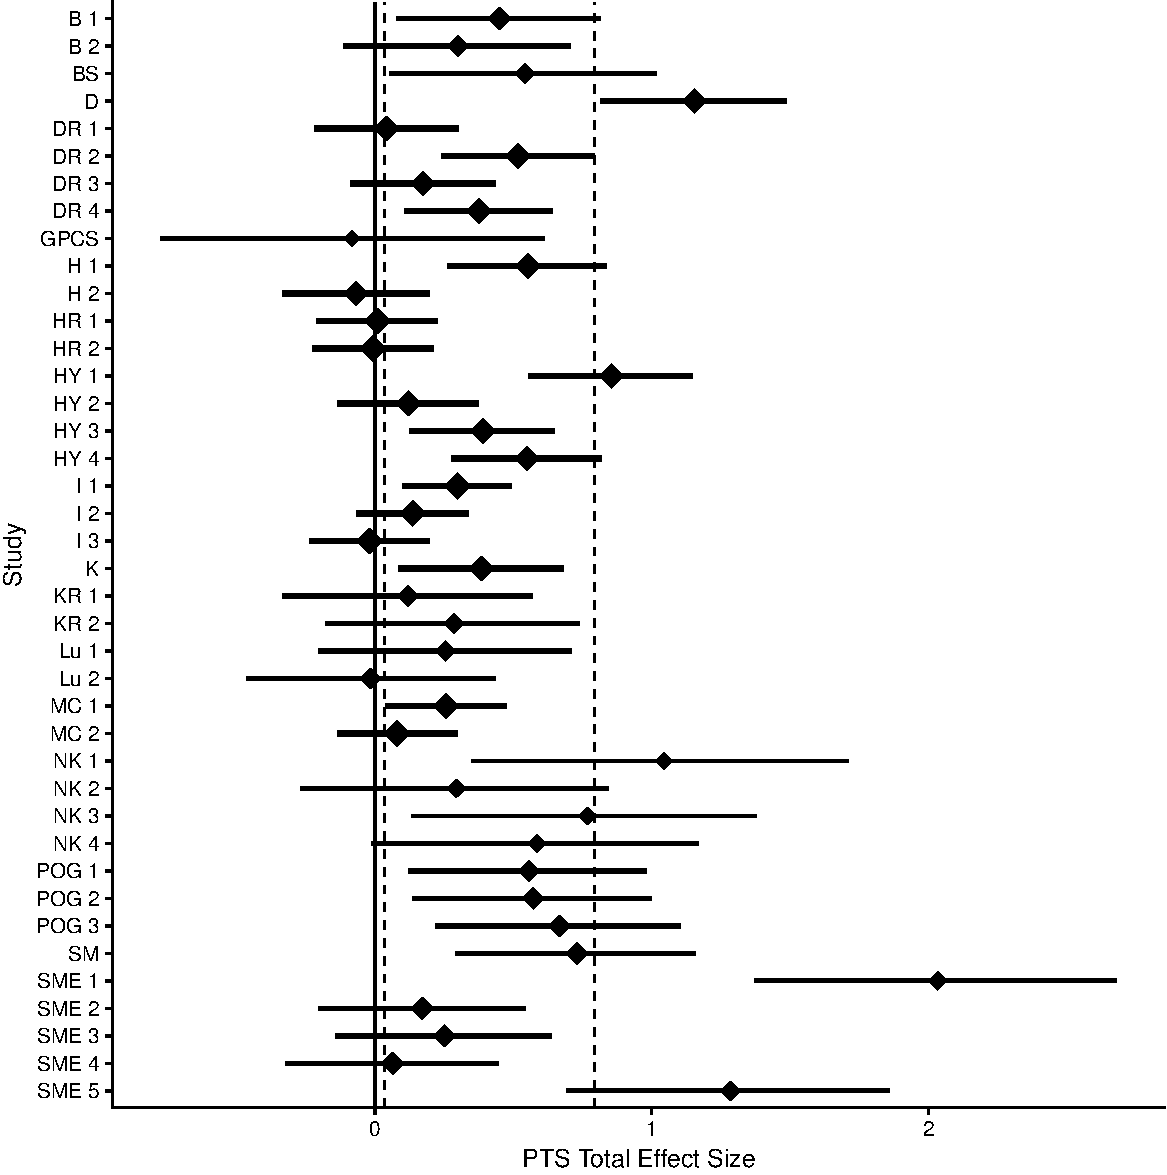
\includegraphics{meta_markdown_files/figure-latex/ptspicoverall-1.pdf}
\caption{\label{fig:ptspicoverall}Effect sizes and their non-centralized
confidence interval for PTS total scores. Dashed lines indicated average
non-weighted lower and upper confidence interval limits. Diamond size
indicates normalized study weight from a random effects model.}
\end{figure}

\begin{figure}
\centering
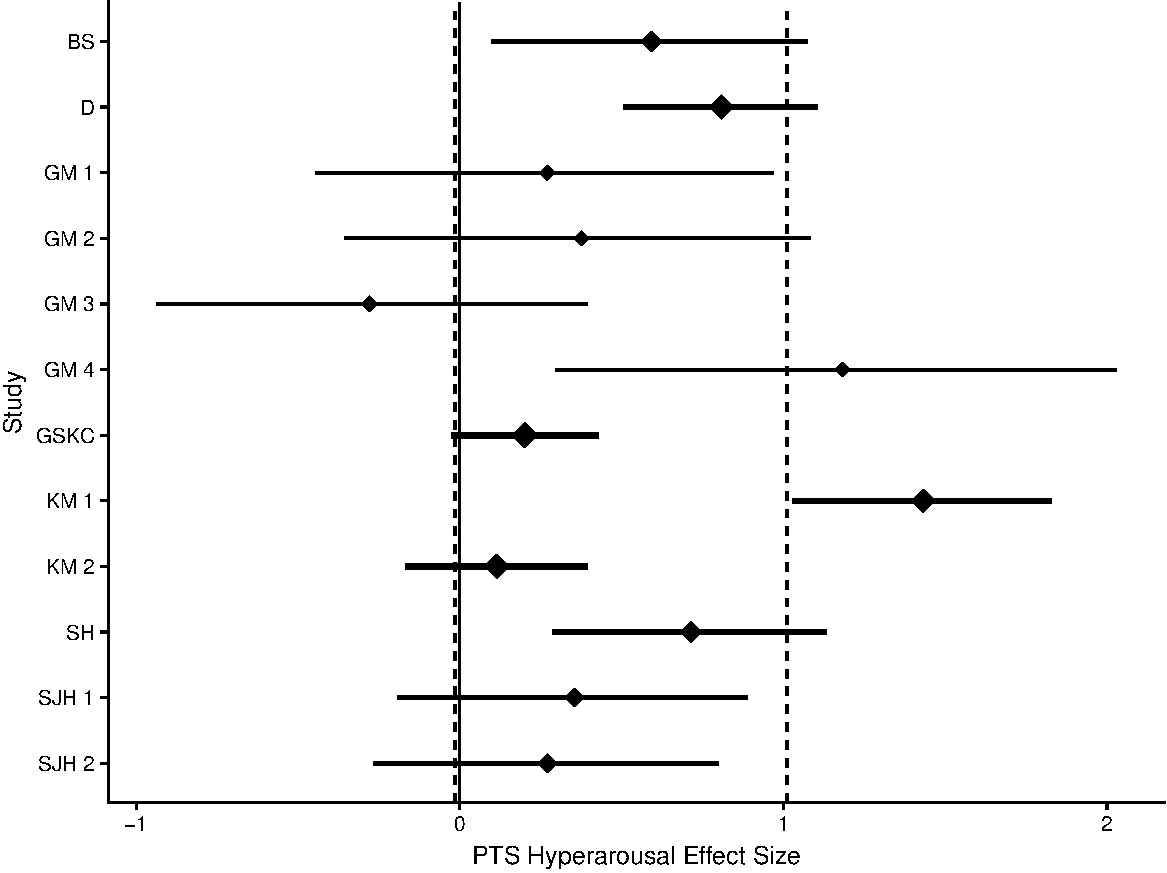
\includegraphics{meta_markdown_files/figure-latex/ptspichyper-1.pdf}
\caption{\label{fig:ptspichyper}Effect sizes and their non-centralized
confidence interval for PTS Hyperarousal. Dashed lines indicated average
non-weighted lower and upper confidence interval limits. Diamond size
indicates normalized study weight from a random effects model.}
\end{figure}

\begin{figure}
\centering
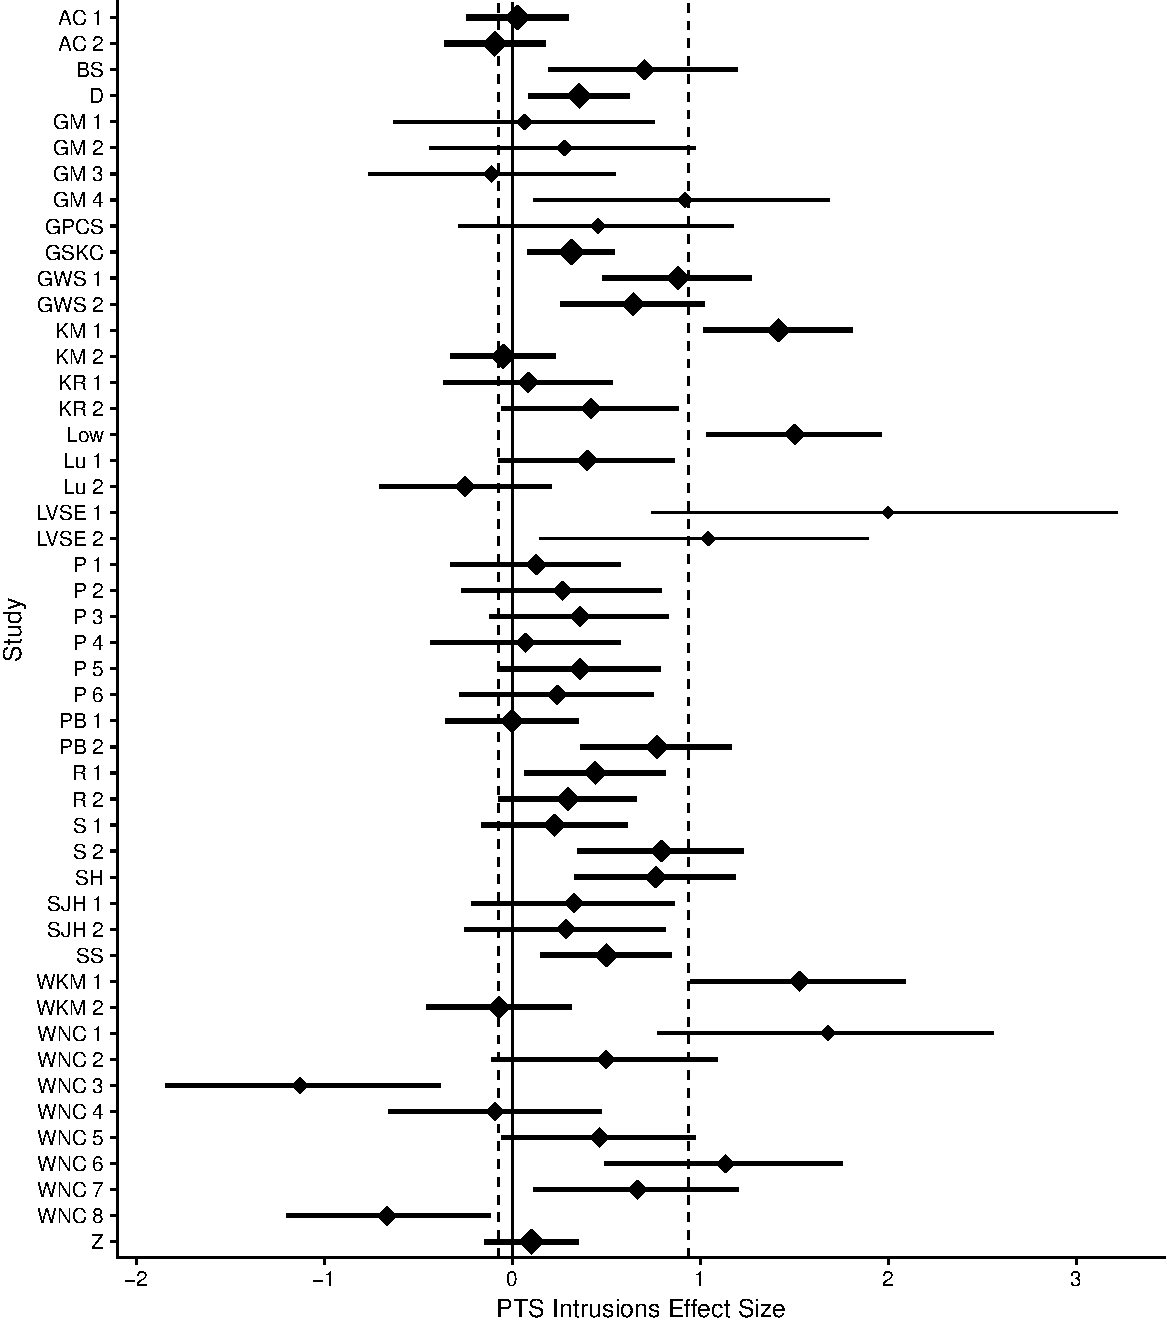
\includegraphics{meta_markdown_files/figure-latex/ptspicint-1.pdf}
\caption{\label{fig:ptspicint}Effect sizes and their non-centralized
confidence interval for PTS Intrusion scores. Dashed lines indicated
average non-weighted lower and upper confidence interval limits. Diamond
size indicates normalized study weight from a random effects model.}
\end{figure}

\begin{figure}
\centering
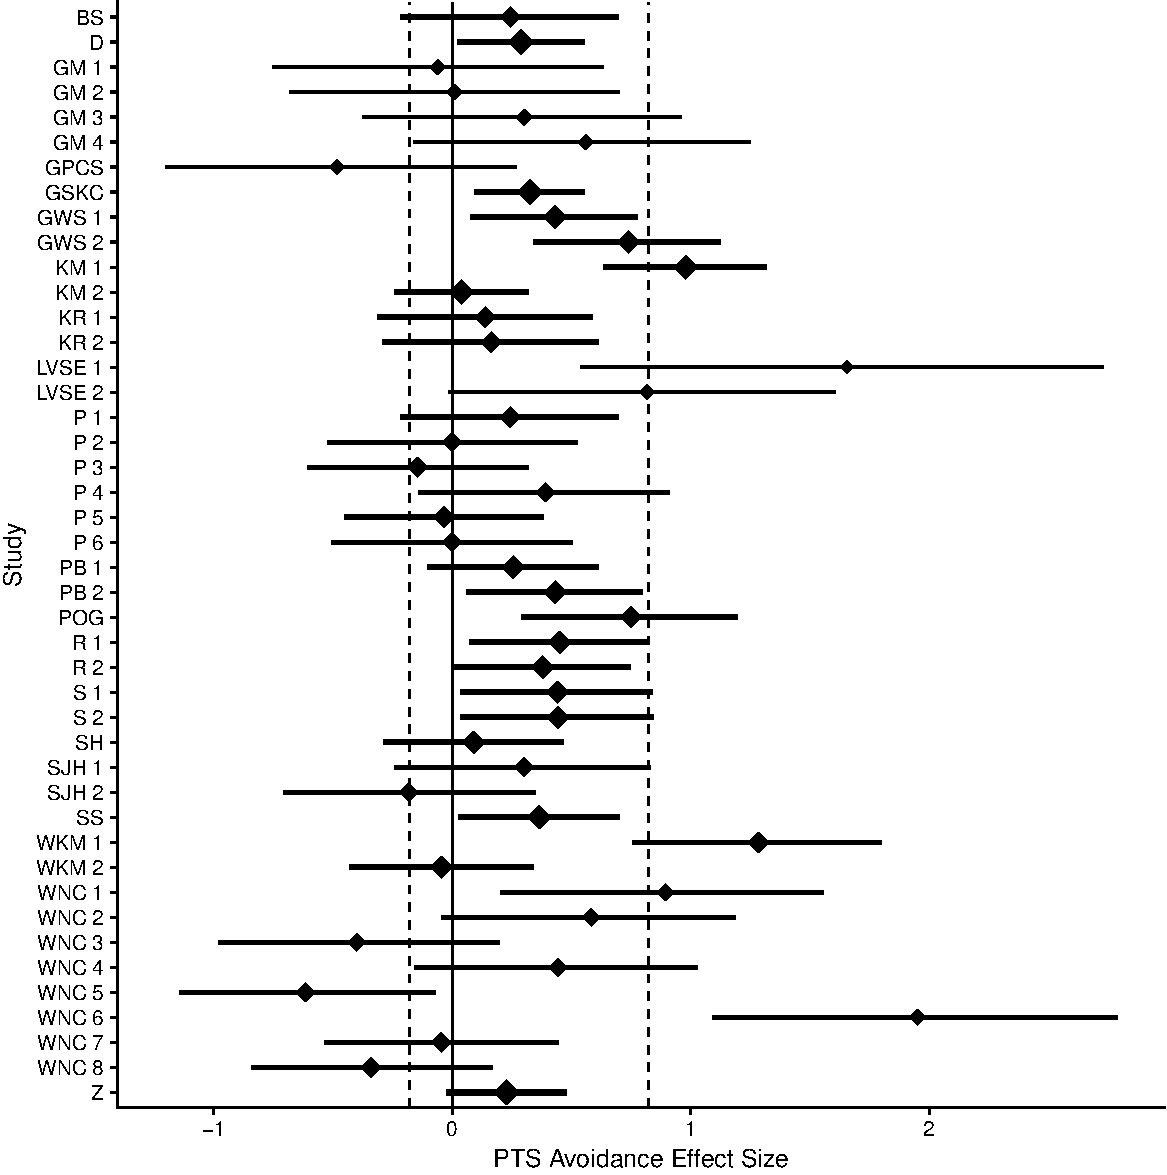
\includegraphics{meta_markdown_files/figure-latex/ptspicavoid-1.pdf}
\caption{\label{fig:ptspicavoid}Effect sizes and their non-centralized
confidence interval for PTS Avoidance Scores. Dashed lines indicated
average non-weighted lower and upper confidence interval limits. Diamond
size indicates normalized study weight from a random effects model.}
\end{figure}

\subsubsection{Homogeneity}\label{homogeneity}

A prerequisite for newer meta-analytic techniques includes the
assessment of homogeneity of the effects \autocite{VanAert2016}. Using
the \emph{metafor} package in \emph{R}, we calculated the
\emph{Q}-statistic and the \(I^2\) index
\autocites{Cochran1954}{Huedo-Medina2006}. Significant values imply
inconsistencies across the variable or variables of interest and are
represented by \emph{Q}. In contrast, \(I^2\) indicates the percentage
of heterogeneity along with a 95\% CI. Both can, however, be biased with
a small number of experiments included for analyses
\autocites{Higgins2003}{Huedo-Medina2006}. Thus, we sought to calculate
an overall level of heterogeneity after examining each variable
separately before and after excluding outliers. For PTS studies
including outliers, we found significant heterogeneity, \emph{Q}(143) =
639.98, \emph{p} \textless{} .001 and \(I^2\) = 77.7, 95\% CI{[}73.9 -
80.9{]}. These values were reduced slightly with the exclusion of
outliers, \emph{Q}(140) = 519.75, \emph{p} \textless{} .001 and \(I^2\)
= 73.1, 95\% CI{[}68.2 - 77.2{]}.

\subsubsection{Power}\label{power}

Power was calculated in two different ways using the \emph{pwr} package
in \emph{R} \autocite{Champely2016}. \emph{Post hoc} power was first
calculated using sample size and effect size statistics from each
individual study. Additionally, we calculated power using the study
sample size and estimated overall effect size from the random effects
model with and without outliers, as explained by \textcite{Francis2012}
and \textcite{Francis2014}. The first estimate indicates the likelihood
of finding an effect from our sample statistics, while the second
indicates the likelihood of finding the true population effect size. If
each study had been conducted on only the change in the experimental
group, 45.1\% of studies would have been considered significant at
\(\alpha\) \textless{} .05. The average power of these studies based on
their original study characteristics was .46 (\emph{SD} = .36). Power
for the random-effects meta-analytic effect size with outliers was .47
(\emph{SD} = .24) and without outliers was .42 (\emph{SD} = .23).
Therefore, power consistently was around 40-50\% for studies examining
PTS, regardless of outlier effects. In these studies, only 26.4\%
achieved recommended 80\% power for their found effect size, a smaller
16.7\% for the random-effect outlier effect size, and even smaller 6.9\%
for power calculations on the random-effect size without the outliers.

\subsubsection{Other Meta-Analytic
Estimates}\label{other-meta-analytic-estimates}

As noted in \textcite{VanAert2016}, \emph{p}-curve and \emph{p}-uniform
analyses are upwardly biased when heterogeneity is high. Therefore, we
use caution when interpreting these analyses on PTS outcomes. As seen in
Table \ref{tab:PTStable}, the estimates for \emph{p}-uniform were higher
than other techniques, likely because of the focus on significant
\emph{p}-values and the great degree of heterogeneity described earlier.
\emph{P}-curve pictures can be found at \url{https://osf.io/4mjqt/}
online, and this analysis indicated evidentiary value at \emph{p}
\textless{} .001. Additionally, the \emph{p}-uniform analysis indicated
that there was likely no publication bias present, \emph{Z} = -5.02,
\emph{p} = 1.000. When examining the PET analysis, we found that the
intercept was significant, which indicated that PEESE was likely a
better estimator of the meta-analytic effect size. PEESE estimates were
lower than the original meta-analytic estimate, but confidence intervals
indicated that the effect is small to medium, and still larger than
zero. Selection models indicated a larger effect size, especially with
the random-effects models, and these effects were influenced by the
outliers found in the published studies. Trim and fill models are shown
in Table \ref{tab:PTStable}, and figures are included online. Nineteen
missing studies were imputed for both models with and without outliers.
Across all these effect size estimates, we found that expressive writing
was likely to decrease PTS symptoms in a small to moderate way. The
correlation of effect size across the time span used in the study from
time one to time two was \(r = -.16\), 95\% CI \([-.32\), \(.00]\),
\(t(142) = -1.99\), \(p = .049\), and \(r = -.15\), 95\% CI \([-.30\),
\(.02]\), \(t(139) = -1.75\), \(p = .082\) without outliers. This result
indicated that the effect of expressive writing decreased across time,
but likely not significantly.

\begin{table}[tbp]
\begin{center}
\begin{threeparttable}
\caption{\label{tab:PTStable}Effect Size Estimates for PTS Results}
\small{
\begin{tabular}{lcccc}
\toprule
Model & Fixed Effects & Random Effects & Fixed No Outliers & Random No Outliers\\
\midrule
Overall Effects & 0.34 [0.31, 0.37] & 0.39 [0.32, 0.46] & 0.32 [0.29, 0.35] & 0.36 [0.29, 0.42]\\
$Z$ Values & 21.75, $p$ < .001 & 11.06, $p$ < .001 & 20.00, $p$ < .001 & 11.03, $p$ < .001\\
$p$-Uniform & 0.60 [0.50, 0.71] & - & 0.57 [0.47, 0.67] & -\\
PET & 0.12 [0.03, 0.21] & - & 0.11 [0.02, 0.20] & -\\
PEESE & 0.25 [0.20, 0.30] & - & 0.23 [0.18, 0.28] & -\\
Selection Models & 0.33 [0.28, 0.37] & 0.45 [0.33, 0.57] & 0.29 [0.24, 0.33] & 0.39 [0.27, 0.50]\\
Trim and Fill & 0.26 [0.23, 0.29] & 0.26 [0.18, 0.34] & 0.25 [0.22, 0.28] & 0.25 [0.18, 0.32]\\
\bottomrule
\addlinespace
\end{tabular}
}
\begin{tablenotes}[para]
\textit{Note.} [] indicates the 95 percent confidence interval for each effect size estimate.
\end{tablenotes}
\end{threeparttable}
\end{center}
\end{table}

\subsection{PTG}\label{ptg}

\subsubsection{Overall Effect Size}\label{overall-effect-size-1}

Both fixed and random effects models with centralized confidence
intervals for PTG are presented in Table \ref{tab:PTGtable}. When
examining expressive writing on PTG, no outliers were detected. Fixed
and random effects estimates are included in Table \ref{tab:PTGtable},
while Figure \ref{fig:ptgpic} shows effect sizes for PTG studies where
shape size indicates the normalized weight of the study. Dashed lines
indicate non-weighted lower and upper confidence intervals for
non-centralized estimates. Overall, PTG studies indicated a negligible
to small effect size across both random and fixed effects models, and
the non-centralized confidence intervals indicated an effect that
crossed zero.

\begin{figure}
\centering
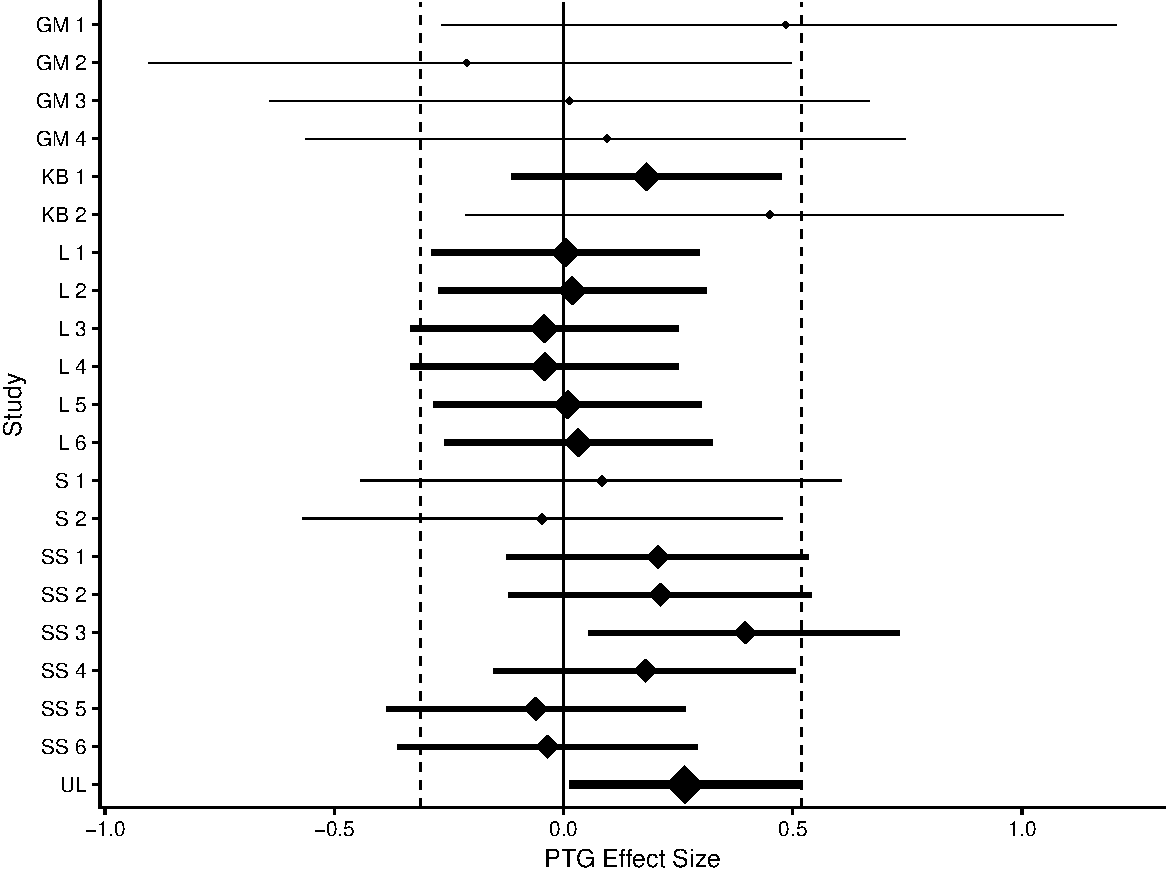
\includegraphics{meta_markdown_files/figure-latex/ptgpic-1.pdf}
\caption{\label{fig:ptgpic}Effect sizes and their non-centralized confidence
interval for PTG outcome variables. Dashed lines indicated average
non-weighted lower and upper confidence interval limits. Diamond size
indicates normalized study weight from a random effects model.}
\end{figure}

\subsubsection{Homogeneity}\label{homogeneity-1}

Using the \emph{metafor} package in \emph{R}, we calculated both a
\emph{Q} statistic and \(I^2\) index. Since PTG studied did not contain
any outliers, we did not calculate two separate analyses to examine
heterogeneity both with and without outliers. We did not find
significant heterogeneity across PTG studies, \emph{Q}(20) = 14.18,
\emph{p} = .82 and \(I^2\) = 0.0, 95\% CI{[}0.0 - 25.3{]}.

\subsubsection{Power}\label{power-1}

First, we calculated \emph{post hoc} power using both sample and effect
size statistics from individual studies. Individual studies examining
change in experimental groups showed that 9.5\% of studies would have
been considered significant at \(\alpha\) \textless{} .05. Average power
of PTG studies was .15 (\emph{SD} = .16). 0.0\% achieved recommended
80\% power for their found effect size. Additionally, we calculated
power using study sample size and estimated effect size from our random
effects model. Power for the true effect size was .08 (\emph{SD} = .02).
Again, 0.0\% achieved recommended 80\% power.

\subsubsection{Other Meta-Analytic
Estimates}\label{other-meta-analytic-estimates-1}

Due to no heterogeneity across PTG studies, we can use both
\emph{p}-curve and \emph{p}-uniform analyses with more confidence. A
pictorial representation of \emph{p}-curve can be found at
\url{https://osf.io/4mjqt/}. This analysis did not indicate evidentiary
value, \emph{p} = .75, as only two of the results would be considered
significant at \(\alpha\) \textless{} .05. \emph{p}-uniform estimates
are presented in Table \ref{tab:PTGtable}. Specifically, these analyses
indicated that there was no publication bias present, \emph{Z} = 0.70,
\emph{p} = .243. The \emph{p}-uniform estimates of the effect size for
PTG were negative, in contrast to the fixed and random effects overall
model. The confidence interval for this analysis indicates a wide range
of possible effects. In examining PET-PEESE analyses, we did not find a
significant intercept, indicating that PET is most likely a better
effect size estimator. PET analyses indicated that the effect size is
negligible to small, with our confidence interval crossing zero. These
results corroborated our original effect size calculations. Selection
models indicated negligible to small effect sizes, again wherein the
confidence interval includes zero effect. Trim and fill models are shown
in Table \ref{tab:PTGtable}, and figures are included online. Zero
studies were imputed for our model, and thus, the effect size estimate
is the same as the overall model. Across techniques, we found that
expressive writing has little to no effect on PTG. The correlation of
effect size across time span used in PTG studies at subsequent time
points was \(r = .09\), 95\% CI \([-.36\), \(.50]\), \(t(19) = 0.38\),
\(p = .707\), and no change over time was found.

\begin{table}[tbp]
\begin{center}
\begin{threeparttable}
\caption{\label{tab:PTGtable}Effect Size Estimates for PTG Results}
\small{
\begin{tabular}{lcc}
\toprule
Model & Fixed Effects & Random Effects\\
\midrule
Overall Effects & 0.10 [0.02, 0.17] & 0.10 [0.02, 0.17]\\
$Z$ Values & 2.45, $p$ = .014 & 2.45, $p$ = .014\\
$p$-Uniform & -0.11 [-1.43, 0.42] & -\\
PET & 0.06 [-0.20, 0.32] & -\\
PEESE & 0.08 [-0.04, 0.20] & -\\
Selection Models & 0.09 [-0.01, 0.18] & 0.09 [-0.03, 0.20]\\
Trim and Fill & 0.10 [0.02, 0.17] & 0.10 [0.02, 0.17]\\
\bottomrule
\addlinespace
\end{tabular}
}
\begin{tablenotes}[para]
\textit{Note.} [] indicates the 95 percent confidence interval for each effect size estimate.
\end{tablenotes}
\end{threeparttable}
\end{center}
\end{table}

\subsection{QOL}\label{qol}

\subsubsection{Overall Effect Size}\label{overall-effect-size-2}

Finally, for QOL, both fixed and random effects models with centralized
confidence intervals are presented in Table \ref{tab:QOLtable}. Two
outliers were detected with this procedure, average \emph{d} = -0.07.
While the average effect of these outliers indicates a small number, it
is important to note that these two outliers were the largest positive
and negative effects found from the \textcite{Possemato2010} study.
Fixed and random effects estimates without these points are also
included in Table \ref{tab:QOLtable}, while Figure \ref{fig:qolpic}
shows effect sizes for QOL studies. Overall, QOL studies indicated a
negligible to small effect that showed a nonsignficant decrease in
quality of life as a result of expressive writing.

\begin{figure}
\centering
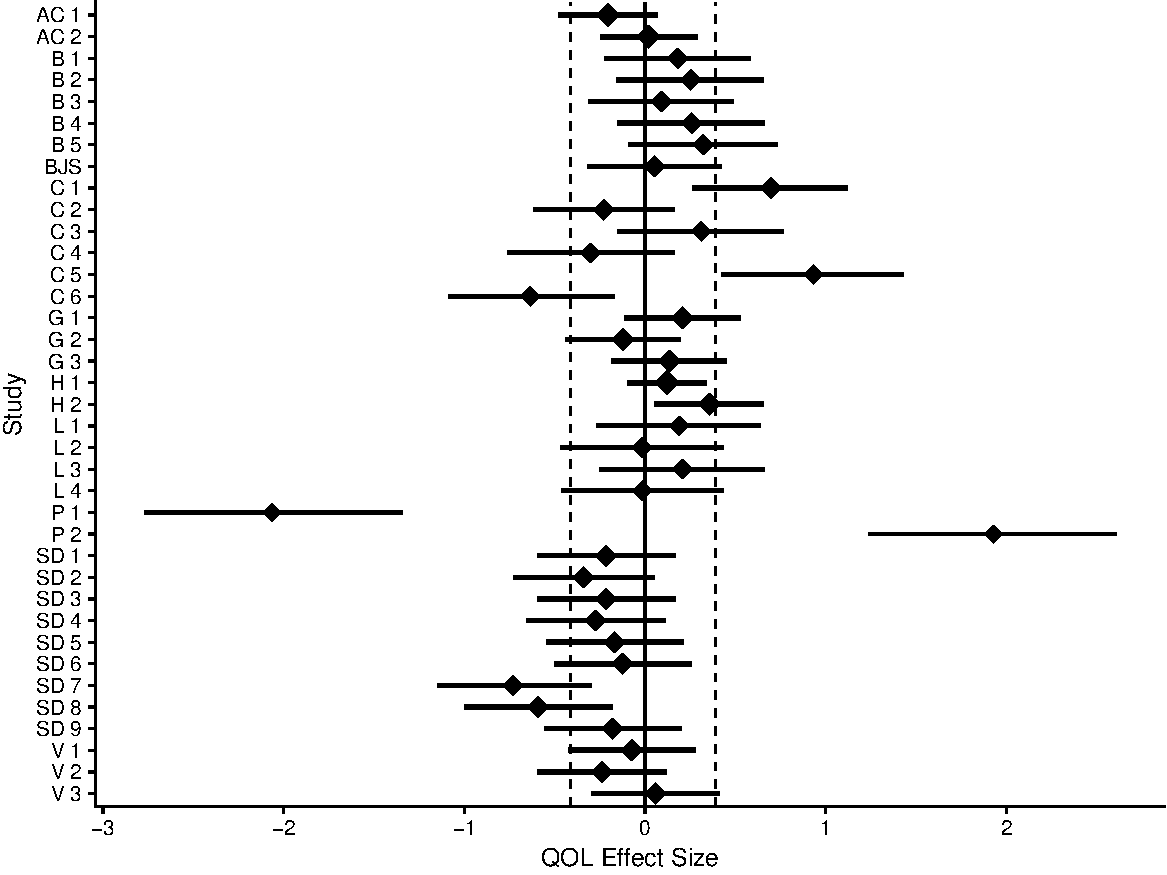
\includegraphics{meta_markdown_files/figure-latex/qolpic-1.pdf}
\caption{\label{fig:qolpic}Effect sizes and their non-centralized confidence
interval for QOL outcome variables. Dashed lines indicated average
non-weighted lower and upper confidence interval limits. Diamond size
indicates normalized study weight from a random effects model.}
\end{figure}

\subsubsection{Homogeneity}\label{homogeneity-2}

For QOL studies including outliers, we found significant heterogeneity
from our random effects model, \emph{Q}(36) = 200.09, \emph{p}
\textless{} .001 and \(I^2\) = 82.0, 95\% CI{[}75.9 - 86.5{]}. After
excluding outliers, our random effects model still indicated
heterogeneity,\emph{Q}(34) = 93.18, \emph{p} \textless{} .001 and
\(I^2\) = 63.5, 95\% CI{[}47.6 - 74.6{]}.

\subsubsection{Power}\label{power-2}

In conducting \emph{post hoc} power using sample and effect size
statistics from individual studies, we found that 21.6\% of studies
would have been considered significant at \(\alpha\) \textless{} .05.
Average power based on actual study characteristics was .33 (\emph{SD} =
.32). Power for the random effects meta-analytic effect size with
outliers was .05 (\emph{SD} = .00) and without outliers was .05
(\emph{SD} = .00). Unfortunately, power was around 5\% for both random
effects models with and without outliers. In these studies, 18.9\%
achieved adequate power of 80\% on their found effect size, while 0.0\%
achieved 80\% power for our random effects model with outliers. Finally,
without outliers, 0.0\% achieved 80\% power.

\subsubsection{Other Meta-Analytic
Estimates}\label{other-meta-analytic-estimates-2}

We exert caution in interpreting \emph{p}-curve and \emph{p}-uniform
analyses on QOL outcomes with and without outliers due to heterogeneity.
As seen in Table \ref{tab:PTStable}, \emph{p}-uniform estimates were
stronger and positive than other techniques because of the high degree
of heterogeneity recently described. \emph{p}-curve pictures can be
found at the following OSF Link: \url{https://osf.io/4mjqt}. Eight
studies were significant at \(\alpha\) \textless{} .05, and the studies
indicated evidentiary value, \emph{p} = .004. \emph{p}-uniform analyses
did not indicate publication bias, \emph{Z} = -2.75, \emph{p} = .997. In
PET-PEESE analyses, we found that the intercept was not significant, and
therefore, PET was a better estimator of the meta-analytic effect. Table
\ref{tab:PTStable} indicates that both of these analyses estimate the
effect size around zero, with a confidence interval that includes zero.
Selection models correspondingly show small effects crossing zero,
except for random effects models with outliers, that appear to be
heavily influenced by the outliers. Trim and fill models are shown in
Table \ref{tab:QOLtable}, and figures are included online. No studies
were imputed for these analyses, and therefore, the effect size
estimates match the original meta-analysis. Overall, these results
appear to point to no effects, ranging across zero with several negative
estimates. Interestingly, the correlation of effect sizes across time
points in this study with outliers was \(r = -.37\), 95\% CI \([-.62\),
\(-.05]\), \(t(35) = -2.33\), \(p = .026\) and \(r = -.64\), 95\% CI
\([-.80\), \(-.39]\), \(t(33) = -4.75\), \(p < .001\) without outliers.
The effect of expressive writing appears to be positive at short time
intervals and decreases into negative effects at longer time intervals.

\begin{table}[tbp]
\begin{center}
\begin{threeparttable}
\caption{\label{tab:QOLtable}Effect Size Estimates for QOL Results}
\small{
\begin{tabular}{lcccc}
\toprule
Model & Fixed Effects & Random Effects & Fixed No Outliers & Random No Outliers\\
\midrule
Overall Effects & -0.01 [-0.07, 0.05] & -0.01 [-0.16, 0.13] & -0.01 [-0.07, 0.05] & -0.01 [-0.11, 0.09]\\
$Z$ Values & -0.33, $p$ = .745 & -0.18, $p$ = .860 & -0.25, $p$ = .805 & -0.20, $p$ = .838\\
$p$-Uniform & 0.79 [0.33, 1.61] & - & 0.62 [0.10, 0.96] & -\\
PET & 0.05 [-0.26, 0.36] & - & 0.05 [-0.29, 0.38] & -\\
PEESE & 0.00 [-0.17, 0.17] & - & 0.00 [-0.19, 0.19] & -\\
Selection Models & -0.06 [-0.12, 0.01] & 0.51 [-0.09, 1.12] & -0.04 [-0.11, 0.03] & 0.05 [-0.15, 0.24]\\
Trim and Fill & -0.01 [-0.07, 0.05] & -0.01 [-0.16, 0.13] & -0.01 [-0.07, 0.05] & -0.01 [-0.11, 0.09]\\
\bottomrule
\addlinespace
\end{tabular}
}
\begin{tablenotes}[para]
\textit{Note.} [] indicates the 95 percent confidence interval for each effect size estimate.
\end{tablenotes}
\end{threeparttable}
\end{center}
\end{table}

\section{Discussion}\label{discussion}

In examining pre- to post-test comparisons across each variable
separately, we found that PTS studies indicated a small effect size
across all meta-analytic estimates. Both QOL and PTG studies indicated a
negligible to small effect size using random effects models. Although
the PTG effect in our overall meta-analysis estimate was significant,
other methods indicate this small effect is likely not different from
zero. QOL was not different from zero, which suggests no effect of
expressive writing on quality of life. Interestingly, these results are
in contrast to \textcite{Sloan2011a}, which suggested that only certain
groups may respond to these interventions. Potentially, the high
heterogeneity may be due to the mixed levels of PTSD in these studies,
as \textcite{Blasio2015a} indicates that only certain levels of PTSD are
responsive to an expressive writing condition.

Expressive writing does not appear to play an important role in
influencing positive growth or improved quality of life post
intervention. Ineffective emotional expression may be a contributing
factor. Additionally, future research might examine specific methodology
for these types of studies. If participants/clients are not deeply
engaged with the material, an expressive writing intervention may not be
effective, as \textcite{Pennebaker2001} imply that connectedness is an
important factor for the intervention. However, it may be difficult to
implement a check for engagement in these types of research designs.
Doing so may also set a context that will inhibit emotional processing
and general responses. Research on expressive writing has found a wide
range of outcomes for different variables \autocite{Frattaroli2006}, and
these various results may explain the large heterogeneity found in this
study. Encouragingly, however, we did not find much evidence of
publication bias, and therefore, these estimates may represent a true
population effect size.

We also examined the relationship of time between measurements of the
dependent variables and the corresponding effect size to determine if
effects change over time. For both PTS and PTG, there was no
relationship between effect size and time; yet, PTS indicated a small
negative correlation. For QOL studies, a medium to large negative
correlation was found. A negative relationship between time and effect
size implies that interventions were more effective in the initial time
points, and effects decreased over longer time spans.

The psychological scientific community has shifted focus to
reproducibility and research design in the last several years
\autocite{Nelson2018}, and much of this discussion has focused on
adequately powering studies for publication
\autocites{Bakker2016}{Maxwell2015}. \textcite{Maxwell2015} and
\textcite{OpenScienceCollaboration2015} have shown that the
\enquote{replication crisis} may be attributed to low power in published
studies. The power found in the current meta-analysis was very poor,
with very few studies reaching the suggested 80\% criterion to
adequately power their study. This result was the same when considering
individual study characteristics or the estimate true population effect
size. Research by \textcite{Bakker2016} indicates that researchers'
intuitions about power are particularly poor, and many studies could
benefit from more informed power analyses. \textcite{Anderson2017a}
recently published a primer on power, with an online application to help
with sample size planning for many types of research designs.
Additionally, we encourage researchers to report power analyses of
studies in order to better understand methodology for replication and
reproducibility.

Meta-analyses, while useful tools to pool for population effect sizes,
contain various limitations to their usefulness \autocite{VanElk2015}.
As mentioned previously, these analyses can be affected by high
heterogeneity, which was found in this study \autocite{VanAert2016}.
Selection models have been criticized when using a smaller number of
studies \autocite{VanAssen2015}, and trim and fill analyses may not
always estimate accurate confidence intervals and funnel plots may be
biased with heterogeneity \autocite{Terrin2003}. When focusing on
improving the psychological sciences, \textcite{VanElk2015} suggest that
the reliability and size of effects may be best elucidated by conducting
large preregistrated studies. This suggestion will also improve the
outlook for power in published studies, and projects such as Many Labs
can aide in subsidizing large samples \autocite{Klein2014a}. Even with
limitations, meta-analyses allow researchers to examine the state of a
research area, and we find potential with expressive writing on reducing
PTS symptoms, and an overall need for better sample size and power
planning for studies.

\newpage

\section{References}\label{references}

\setlength{\parindent}{-0.5in} \setlength{\leftskip}{0.5in}

  \printbibliography





\end{document}
